\documentclass{beamer}
\usepackage{amsmath}
\usepackage{ctex}
\usepackage{xcolor}
\usepackage{geometry}
\usepackage{amssymb}
\usepackage{bm}
\usepackage{pgf}
\usepackage{tikz}
\usepackage{subfigure} 
\usepackage{graphicx}
\usepackage{fontspec}
\usepackage{multicol}
\usepackage[backend=biber,style=numeric,sorting=none]{biblatex}
\usetheme[height=7mm]{Rochester}
\usecolortheme{rose}
\setbeamertemplate{footline}[frame number]
\usefonttheme[onlylarge]{structurebold}
\usefonttheme[onlymath]{serif}
\setCJKsansfont{KaiTi}[AutoFakeBold]
\setbeamertemplate{navigation symbols}{}
\usepackage{multicol} 

\setlength\columnsep{-1cm}
\newtheorem{assumption}{假设}
% \setsansfont{Fontin-SmallCaps}
% \setbeamerfont{title}{shape=\itshape,family=\rmfamily}
% \setbeamerfont{frametitle}{family=\rmfamily,series=\bfseries}


\setbeamerfont{footnote}{size=\tiny} %调整注脚的文字大小
\setbeamertemplate{theorems}[numbered]
\title{Tractable Approximate Counting for CQs}

% \titlegraphic{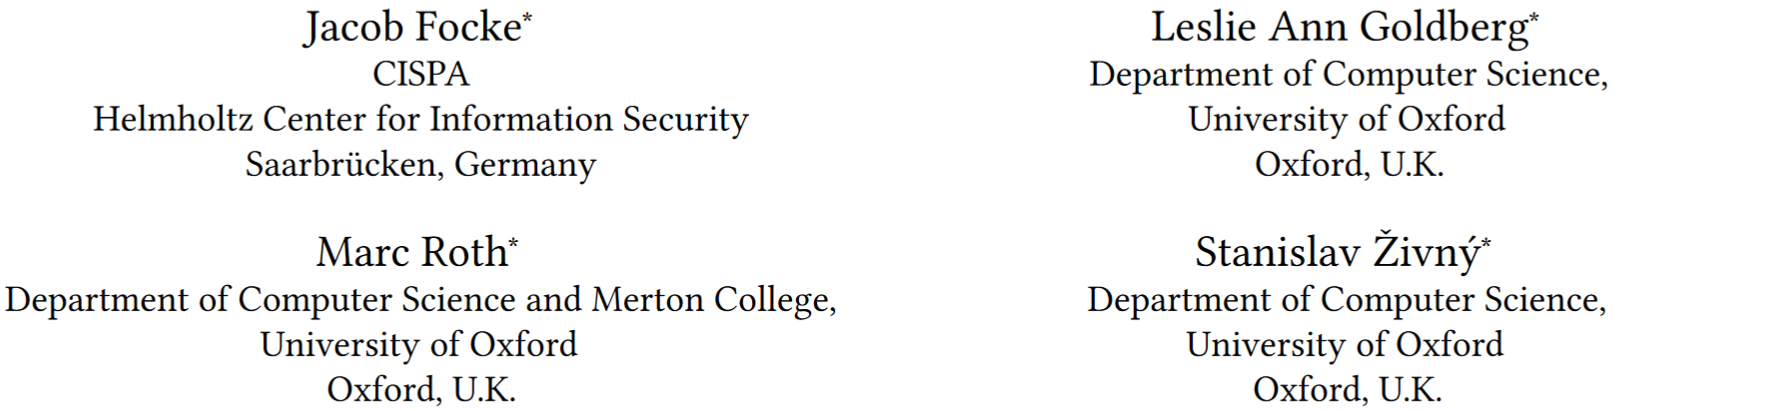
\includegraphics[width=\textwidth]{pics/title}}
\author{\textbf{报告人:陈鹏宇}}
\institute{\textbf{哈尔滨工业大学}}
\date{\today}
\AtBeginSection[]
{
	\begin{frame}{Content}
        % \begin{multicols}{1}
		\transfade%淡入淡出效果
		\tableofcontents[sectionstyle=show/shaded,subsectionstyle=show/shaded]
		\addtocounter{framenumber}{-1}  %目录页不计算页码
        % \end{multicols}
	\end{frame}
}
\newcommand{\pic}[2][100]{
	\begin{figure}
		\centering
		\includegraphics[width= #1 mm]{#2}
	\end{figure}
}
\newcommand{\picframe}[3][100]{
	\begin{frame}
		\frametitle{#2}
		\pic[#1]{#3}
	\end{frame}
}
\begin{document}
	\frame{\titlepage}
	\section{Conjunctive Queries}
	\begin{frame}{Conjunctive Query (CQ)}
		\pic{pics/CQ}
	\end{frame}
	\begin{frame}
		\frametitle{Conjunctive Query Complexity}
		\pic{pics/scq}
	\end{frame}

	
	\section{Tree Decomposition and Treewidth}
	\begin{frame}{Tree Decomposition}
		\pic{pics/treewidthdef}
		\begin{example}[Treewidth=2]
				\vspace{-2ex}
			\begin{multicols}{2}
				\centering
				$
				\begin{aligned}
					\varphi(x_1,x_5,x_6)\leftarrow&R_1(x_1,x_2),\\
					&R_2(x_2,x_3,x_4),\\
					&R_3(x_3,x_5),\\
					&R_4(x_4,x_6)
				\end{aligned}
				$
				\newcolumn
				\centering
				\pic[40]{pics/ExampleCQ}
			\end{multicols}
		\vspace{-2ex}
		\end{example}
	\end{frame}
	
	\picframe{Tree Decomposition}{pics/treed}
	\picframe{Tree Width}{pics/treewidth}
	\begin{frame}
		\frametitle{Tree Width}
		\pic[28]{pics/graph}
		\vspace{-4ex}
		\pic{pics/tw32}
	\end{frame}
	\picframe{Tree Width via Games}{pics/twgame}
	\begin{frame}
		\frametitle{Tree Width via Games}
		\begin{figure}
			\centering
			\subfigure{
				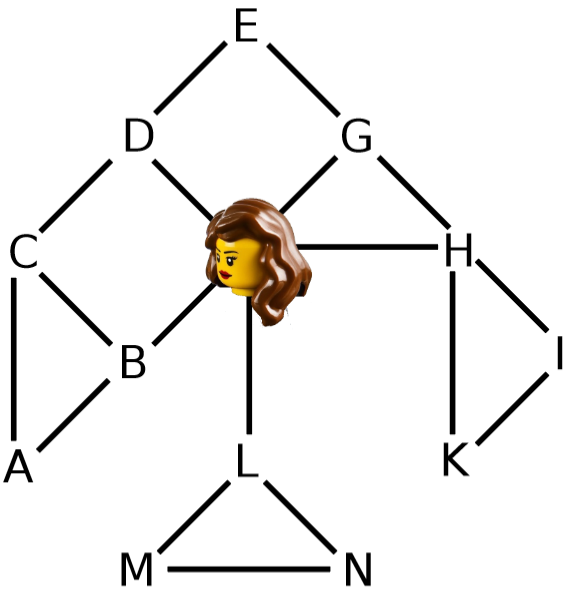
\includegraphics[width= 30 mm]{pics/twgame1}
			}
			\subfigure{
				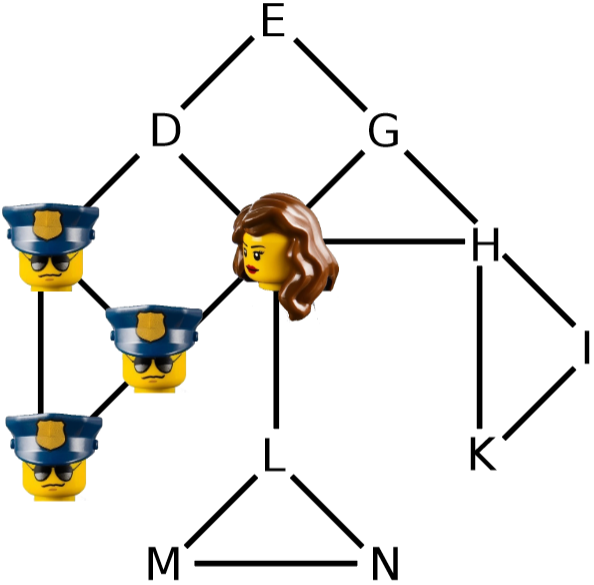
\includegraphics[width= 30 mm]{pics/twgame2}
			}
			\subfigure{
				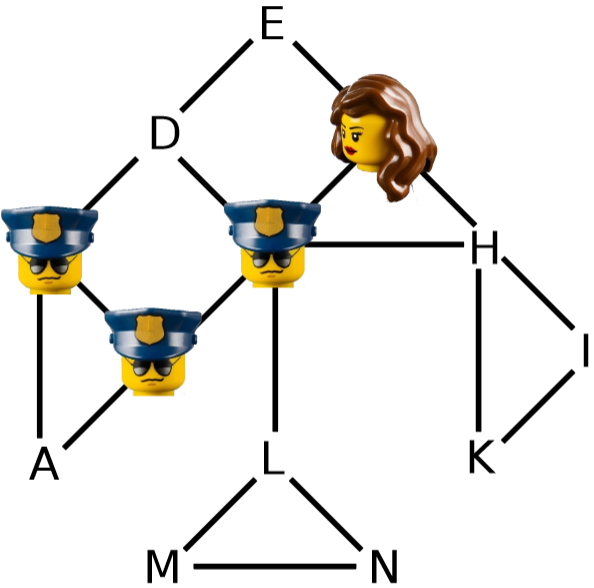
\includegraphics[width= 30 mm]{pics/twgame3}
			}
		\end{figure}
		\vspace{-3ex}
		\begin{figure}
			\centering
			\subfigure{
				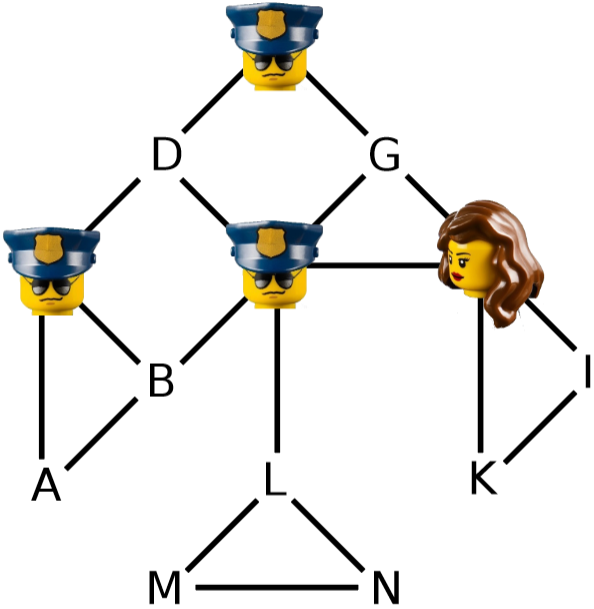
\includegraphics[width= 30 mm]{pics/twgame4}
			}
			\subfigure{
				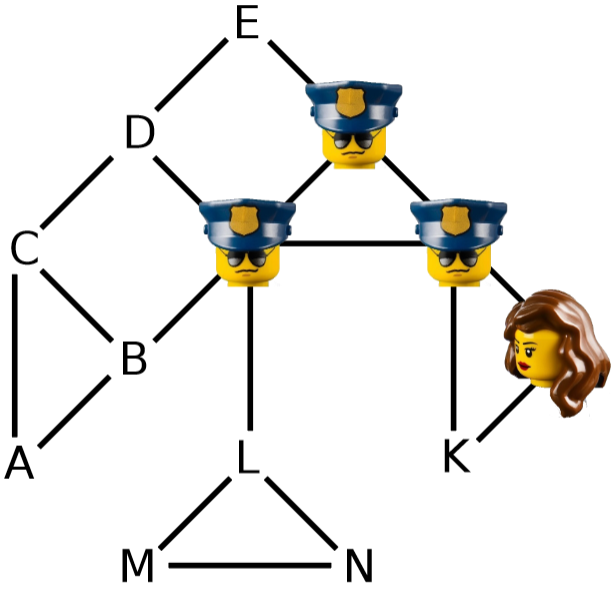
\includegraphics[width= 30 mm]{pics/twgame5}
			}
			\subfigure{
				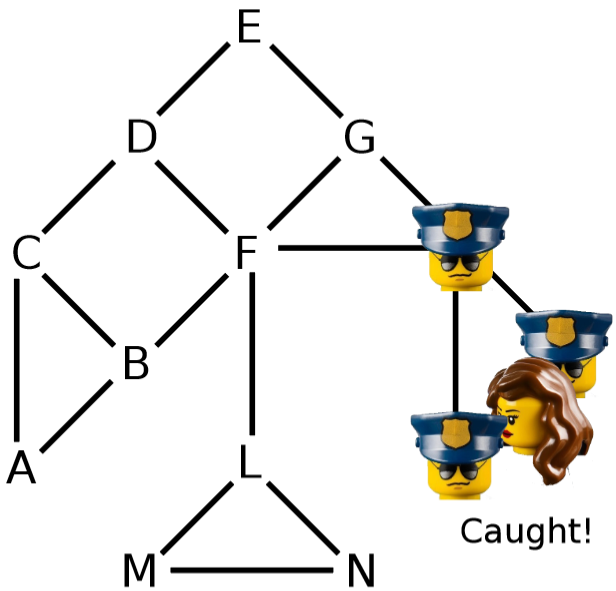
\includegraphics[width= 30 mm]{pics/twgame6}
			}
		\end{figure}
		\vspace{-2ex}
		\pic{pics/twgamethm}
	\end{frame}
	\picframe{Summary of Tree Width}{pics/negfortw}
	\section{Hypertree Decomposition and Hypertreewidth}
	\begin{frame}
		\frametitle{Query Width}
		\pic{pics/qw}
		\vspace{-2ex}
		\pic{pics/hardqw}
	\end{frame}
	\begin{frame}
		\frametitle{Hyper Tree Decomposition\footnotemark}
		\vspace{-2ex}
		\pic{pics/htwdef}
		\vspace{-2ex}
		\begin{example}[Treewidth=2, Hyperwidth=1]
			\vspace{-2ex}
		\begin{multicols}{2}
			\centering
			$
			\begin{aligned}
				\varphi(x_1,x_5,x_6)\leftarrow&R_1(x_1,x_2),\\
				&R_2(x_2,x_3,x_4),\\
				&R_3(x_3,x_5),\\
				&R_4(x_4,x_6)
			\end{aligned}
			$
			\newcolumn
			\centering
			\pic[40]{pics/ExampleCQ2}
		\end{multicols}
	\vspace{-2ex}
	\end{example}
	\footnotetext[1]{(2) is the “special condition”: without it we get the generalized hypertree width}
	\end{frame}
	\begin{frame}
		\frametitle{(Generalized) Hyper Tree Decomposition}
		\vspace{-1ex}
		\begin{figure}
			\centering
			\subfigure{
				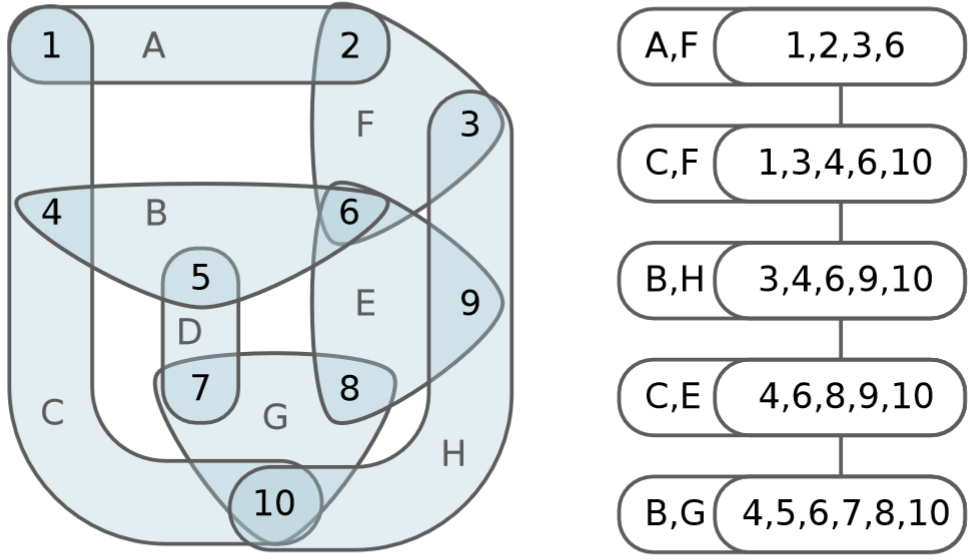
\includegraphics[width= 43 mm]{pics/htw0}
			}
			\subfigure{
				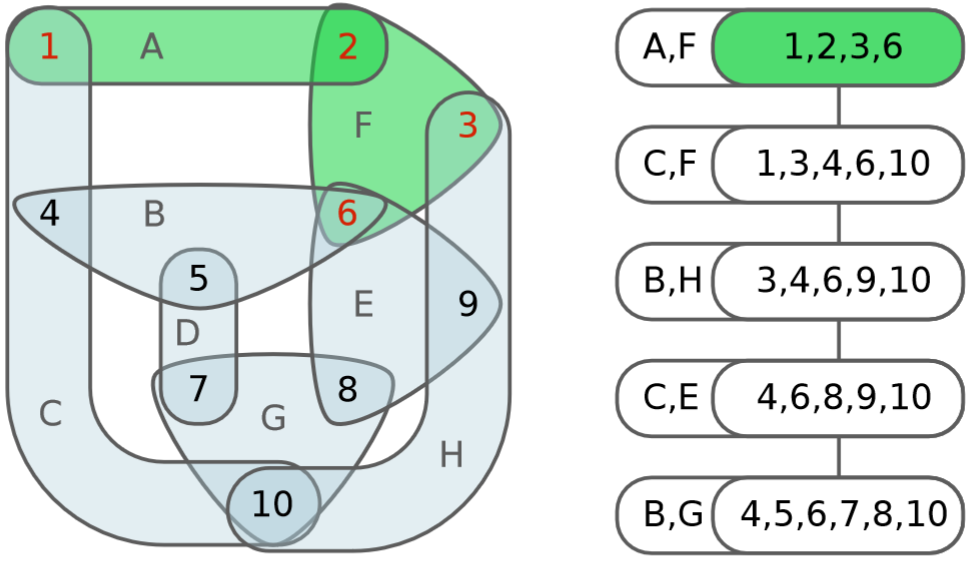
\includegraphics[width= 43 mm]{pics/htw1}
			}
		\end{figure}
		\vspace{-3ex}
		\begin{figure}
			\centering
			\subfigure{
				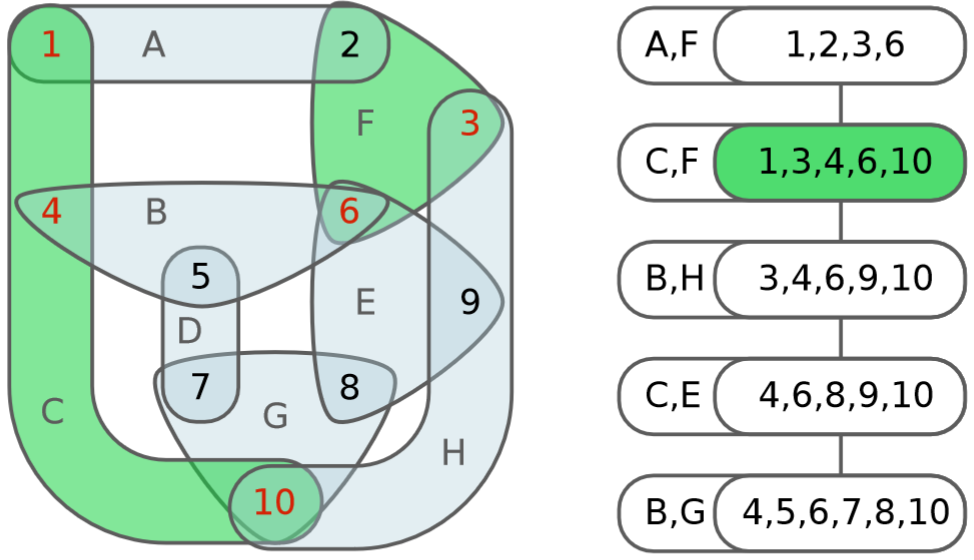
\includegraphics[width= 43 mm]{pics/htw2}
			}
			\subfigure{
				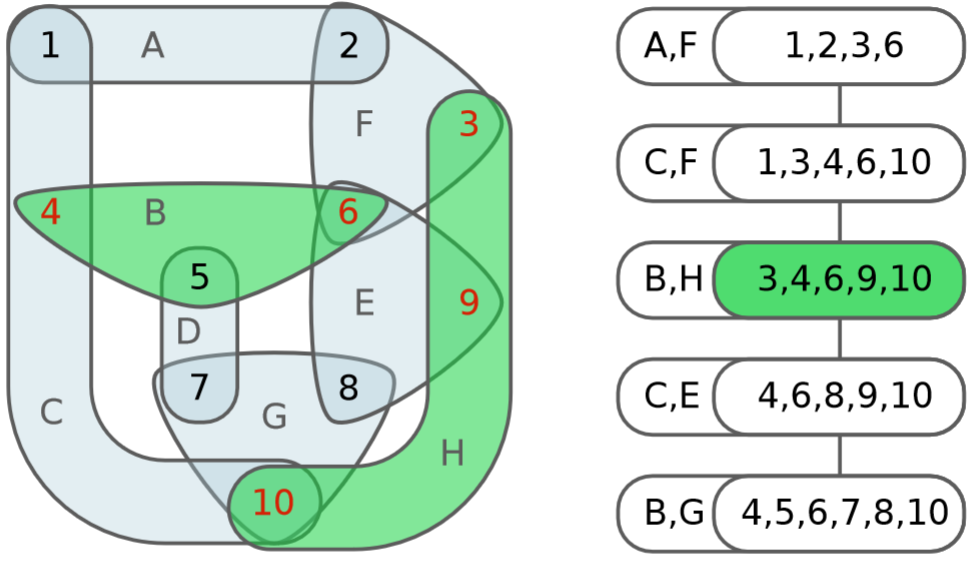
\includegraphics[width= 43 mm]{pics/htw3}
			}
		\end{figure}
		\vspace{-3ex}
		\begin{figure}
			\centering
			\subfigure{
				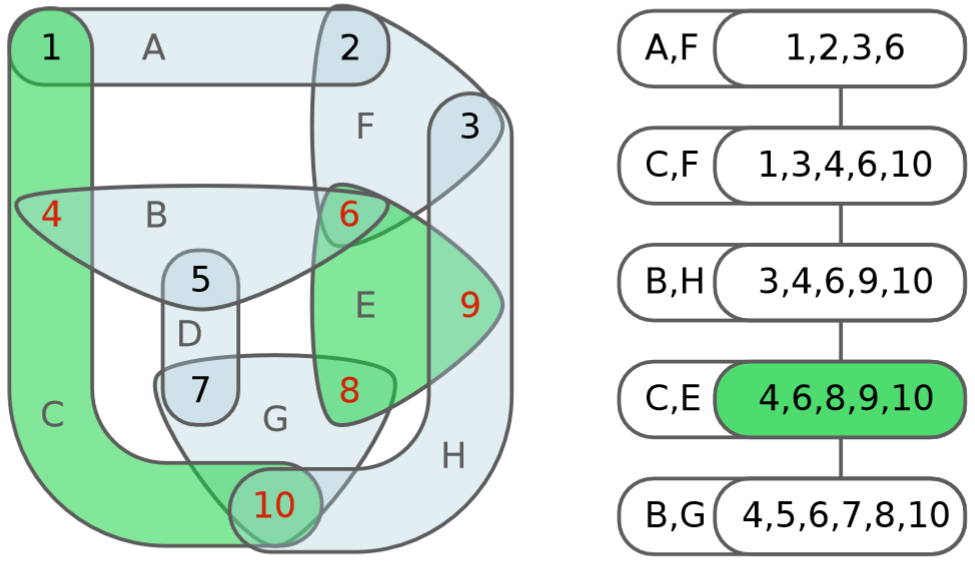
\includegraphics[width= 43 mm]{pics/htw4}
			}
			\subfigure{
				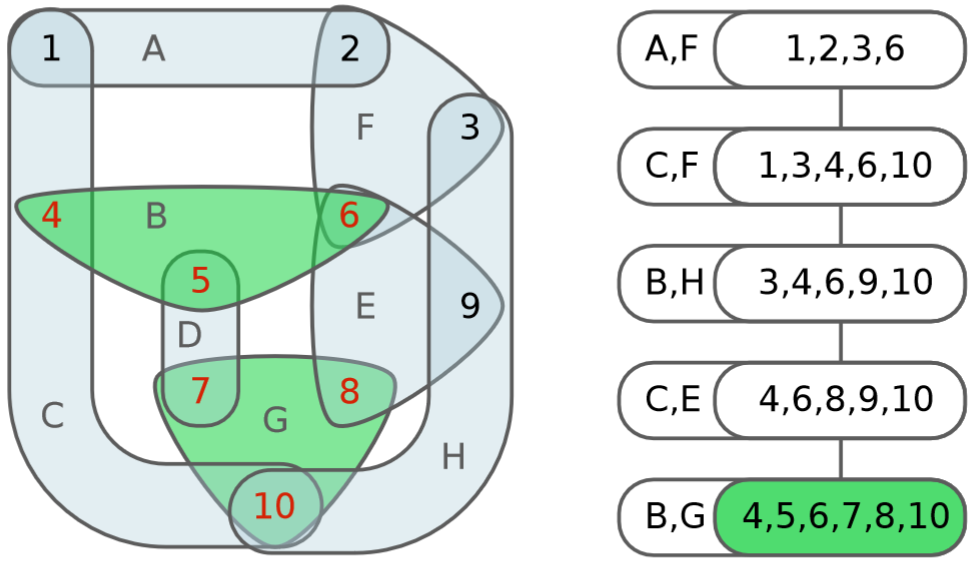
\includegraphics[width= 43 mm]{pics/htw5}
			}
		\end{figure}
		\vspace{-2ex}
	\end{frame}
	\begin{frame}
		\frametitle{(Generalized) Hyper Tree Decomposition}
		\pic[60]{pics/ghw}
		\vspace{-2ex}
		\pic[60]{pics/hww}
	\end{frame}
	\picframe{(Generalized) Hyper Tree Results}{pics/hwresult}

	\picframe{Summary of (Hyper) Tree Width}{pics/tw}
	% \begin{frame}{Main Problems}
	% 	\begin{problem}[\#DCQ, \#ECQ]
	% 		\pic[100]{pics/ECQ}
	% 		\begin{itemize}
	% 			\item \#CQ、\#DCQ的定义与之类似
	% 		\end{itemize}
	% 	\end{problem}
	% 	\begin{definition}[FPRAS,FPTRAS]
	% 		\begin{itemize}
	% 			\item 都是$|\mathrm{Ans}(\varphi,\mathcal{D})|$的$(\varepsilon,\delta)$-近似算法
	% 			\item FPRAS\footnote{fully polynomial randomised approximation scheme}:时间为$\mathrm{poly}(|\mathcal{D}|+|\varphi|,\varepsilon^{-1},\log\delta^{-1})$
	% 			\item FPTRAS\footnote{fixed-parameter tractable randomised approximation scheme}:时间为$f(|\varphi|)\cdot\mathrm{poly}(|\mathcal{D}|,\varepsilon^{-1},\log\delta^{-1})$
	% 		\end{itemize}
	% 	\end{definition}
	% \end{frame}
	\section{Main Results}
	\begin{frame}{Main Results}
		\pic{pics/mainthm}
		\pic{pics/proofapproach}
		\begin{itemize}
			\item FPRAS\footnote{fully polynomial randomised approximation scheme}:时间为$\mathrm{poly}(|\mathcal{D}|+|\varphi|,\varepsilon^{-1},\log\delta^{-1})$
			\item FPTRAS\footnote{fixed-parameter tractable randomised approximation scheme}:时间为$f(|\varphi|)\cdot\mathrm{poly}(|\mathcal{D}|,\varepsilon^{-1},\log\delta^{-1})$
		\end{itemize}
	\end{frame}
	\begin{frame}{Main Results}
		\pic{pics/results}
		\vspace{-1ex}
		\begin{itemize}
			\item \textcolor{orange}{橙色}:宽松条件下的复杂性下界
			\item \textcolor{red}{红色}:\#DCQ、\#ECQ的{\tiny(参数化)}算法及复杂性下界
			\item \textcolor{blue}{蓝色}:\#CQ的{\tiny(FPRAS)}算法及复杂性下界 
		\end{itemize}
	\end{frame}
	\section{From Conjunctive Query to Tree Automata}
	\begin{frame}{Tree Automata (TA)}
		\pic{pics/treeautomata}
		\pic{pics/taexample}			
	\end{frame}
	\begin{frame}{From Conjunctive Query to Tree Automata}
		\pic{pics/cq2ta}
		\vspace{2ex}
		\begin{itemize}
			\item $Q(x)\leftarrow G(x), E(x, y), E(x, z), C(y), M(z)$
		\end{itemize}	
		\vspace{2ex}
		\pic{pics/anstree}		
	\end{frame}
	\section{Counting Accepted Trees of Tree Automata}
	\begin{frame}
		\frametitle{Counting via Sampling}
		\pic{pics/dp}
	\end{frame}
	\picframe{Counting via Sampling}{pics/sample}
	\picframe{Summary and Open Problem}{pics/cfg}
\end{document}